\documentclass{article}

\usepackage[a4paper,pdftex]{geometry}										% A4paper margins
\setlength{\oddsidemargin}{5mm}												% Remove 'twosided' indentation
\setlength{\evensidemargin}{5mm}

\usepackage[english]{babel}
\usepackage[protrusion=true,expansion=true]{microtype}	
\usepackage{amsmath,amsfonts,amsthm,amssymb}
\usepackage{graphicx}
\usepackage{color}
\usepackage{multirow}
\usepackage{rotating}
\usepackage{caption}
\usepackage{subcaption}
\usepackage{verbatimbox}
%\usepackage[parfill]{parskip}

% ------------------------------------------------------------------------------
% Definitions (do not change this)
% ------------------------------------------------------------------------------
\newcommand{\HRule}[1]{\rule{\linewidth}{#1}} 	% Horizontal rule

\makeatletter							% Title
\def\printtitle{%						
    {\centering \@title\par}}
\makeatother									

\makeatletter							% Author
\def\printauthor{%					
    {\centering \large \@author}}				
\makeatother							

% ------------------------------------------------------------------------------
% Metadata (Change this)
% ------------------------------------------------------------------------------
\title{	\textbf{Computer Networks Practicum}
		}

\author{
		Dimo Stoyanov \& Plamen Dimitrov\\
		dsv200 \& pdv200 \\
		Vrije Universiteit Amsterdam\\	
  %      \texttt{your@email.com} \\
}


\begin{document}
% ------------------------------------------------------------------------------
% Maketitle
% ------------------------------------------------------------------------------
\maketitle

\section{Building a TCP stack}
Our TCP implementation follows strictly the RFC0793 except for the differences explicitly
mentioned in the course requirements.

Our implementation does not support multiplexing, therefore only one Socket can be created
per TCP instance. A new Socket can be created if there is no Socket created by the corresponding
TCP instance or if the Socket created by that TCP is in \textit{closed} state.

\subsection{TCP Packet}
The TCPPacket class (See~\ref{fig:tcppacket}) was used to wrap a TCP packet. As can be seen
on Figure~\ref{fig:header}, the class implementation matches exactly the header. The class
also has a method for extracting the relevant information from the payload of an IP Packet.

\begin{figure}[h!]
\centering
\begin{subfigure}[b]{0.4\textwidth}
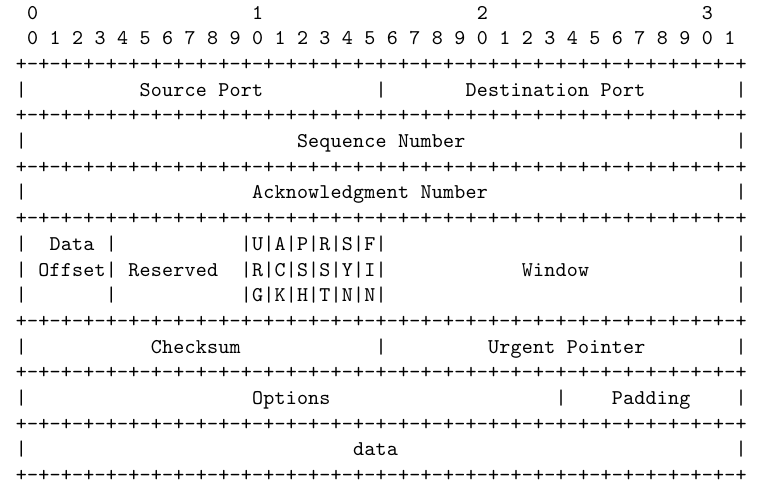
\includegraphics[width=\textwidth]{images/tcp_header}
\caption{TCP header}
\end{subfigure}
\qquad
\begin{subfigure}[b]{0.2\textwidth}
 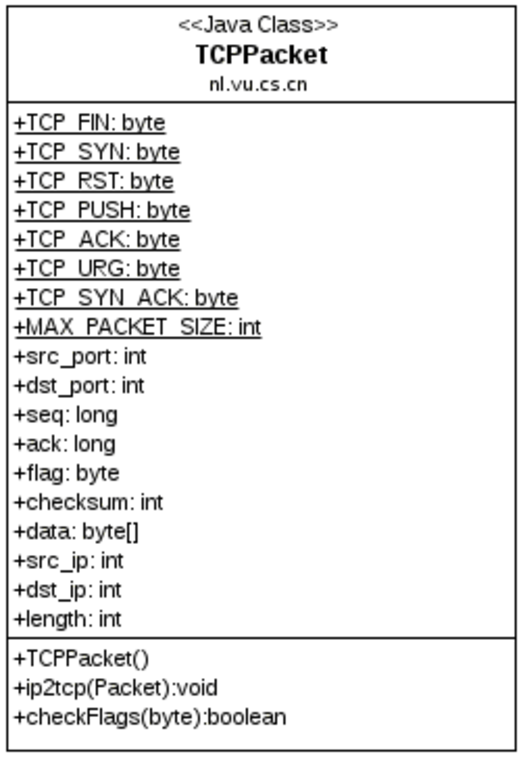
\includegraphics[width=\textwidth]{images/cn_uml}
 \caption{TCPPacket class}
 \label{fig:tcppacket}
\end{subfigure}
\caption{The TCP header and the class used to implement it.}
\label{fig:header}
\end{figure}
\noindent
The types of the TCPPacket's attributes were chosen to adequately represent their ranges and compensate
for the lack of the appropriate unsigned types in Java.
  
\subsection{TCPControlBlock class}
The TCPControlBlock (see Figure~\ref{fig:tcb}) is used to maintain all the information which is needed
for the Socket functioning. The state of the socket is stored in the control block. Figure~\ref{fig:tcb}
shows all the states in our implementation; we will not discuss them in details since they are used
exactly in the way RFC0793 defines them. A socket is uniquely defined based on the control block information.


\begin{figure}[h!]
\centering
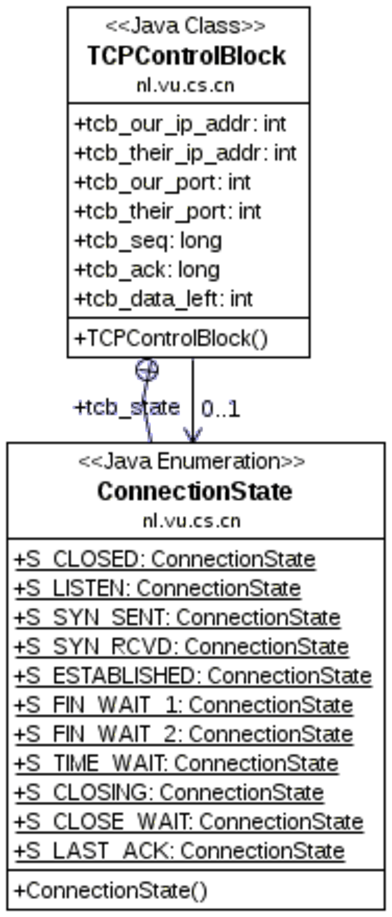
\includegraphics[width=0.2\textwidth]{images/control_block}
\caption{TCPControlBlock class}
\label{fig:tcb}
\end{figure}
  
\subsection{Socket class}
The actual heavy lifting is done in the Socket(see Figure~\ref{fig:socket}) class. As suggested in the assignment, two methods 
(e.g. \textit{send\_tcp\_packet()} and \textit{recv\_tcp\_packet()}) added to the original ones. They carry out the communication
between a socket and the underlying IP layer. The \textit{send\_tcp\_packet()} encodes a TCPPacket into a byte array,
sets the required flags (i.e. sets the PSH flag, usents the URG and RST flags), computes checksums, and transmits the
packet. That method can perform both blocking and non-blocking send. Its non-blocking version is latter 
used for time out detection. The \textit{recv\_tcp\_packet()} method does exactly the opposite to the \textit{send\_tcp\_packet()}:
it receives a packet from the IP layer, checks if the checksum is correct and passes it to the socket
as an instance of the TCPPacket class. If a packet is corrupted (e.g. the checksum calculated from that packet is not 0),
\textit{recv\_tcp\_packet} returns false and therefore its caller has to wait for a retransmit.


\begin{figure}[h!]
 \centering
 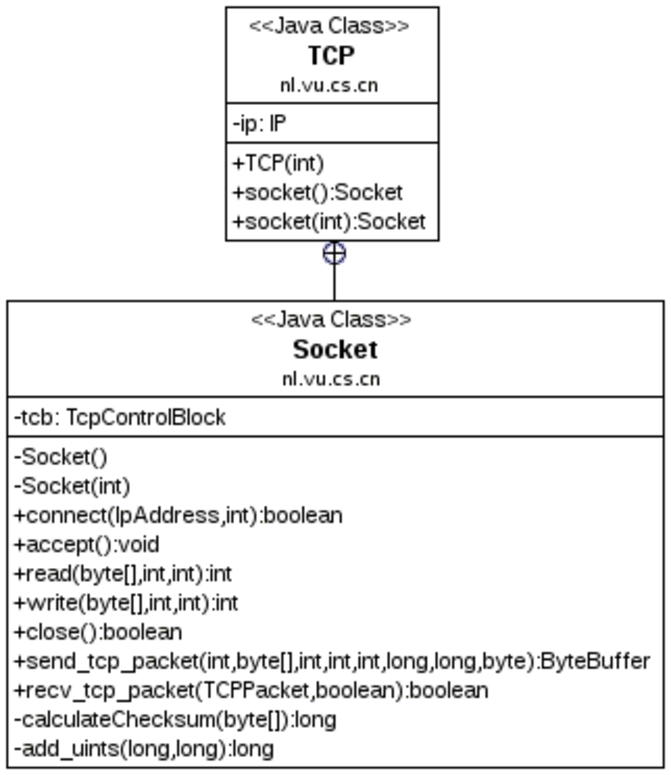
\includegraphics[width=0.5\textwidth]{images/tcp_socket}
 \caption{The TCP and Socket classes}
  \label{fig:socket}
\end{figure}

Another helper method implemented in the Socket class is the \textit{add\_uints()}, used for modular addition of unsigned 32-bit
integers. These integers are represented as longs (64-bit in Java) and the method prevents the addition/subtraction to
cause overflow or underflow of the 32-bit unsigned integer range. That method is used for the change of the sequence
and acknowledgement numbers. 

The main methods in the Socket class are \textit{connect(), accept(), read(), write(), close()}. They have one main feature
in common - the way they deal with errors. To accomplish that, we implemented the state machine from RFC0793. All the methods
require acknowledgement by the other side of every octet they send. In our implementation acknowledgements are sent only in
packets that do not contain any data. The connection between two parties is established by the the \textit{accept()} and
\textit{connect()} methods, which make the standard 3-way handshake.


% Our implementation does not support acknowledgement packets
% carrying data.

The \textit{acept()} method waits for a connection on a given port. When a connection arrives, it changes its state to \textit{syn\_rcvd},
as described in the TCP state machine. \textit{accept()} determines its sequence number randomly from the set of unsigned 32-bit integers.
Afterwards it sends a SYN\_ACK packet to the other party and aways its acknowledgement for maximum of 10 seconds. If an acknowledgement
is received the socket changes its state to \textit{established}, otherwise the state becomes \textit{listen} and the accept is ready
for a new connection.

The \textit{connect()} method, as required, is non-blocking and connects a client socket to a server on given \textit{host}
and \textit{port}. The \textit{connect} first determines randomly, in the range of the 32-bit unsigned integers,
the sequence number it is going to use. As part of the standard 3-way handshake, \textit{connect()} sends a SYN packet,
changes its state to \textit{syn\_sent} and waits for 10 seconds for a SYN\_ACK packet. If such a packet is received, an acknowledgement
is sent, the state is changed to \textit{established} and it returns true. In any other case \textit{connect()} returns false. It also
returns false if it is unable to sent the packets.

The \textit{read()} method blocks until it receives data. The first thing it does is to check if the socket is in one of the appropriate states
according to the TCP state machine. After the first packet receipt \textit{read()} reads data until the total amount
reaches a MAXLEN value or no packet is received in a time period of 10 seconds. 



\section{The Chat Application}
A minimalistic chat application was developed on top of the TCP stack described in the previous chapter.
It consists of a single window used by both a client and a server. The server waits for a connection
(e.g. accepts) and the client connects to the server. Because of the lack of multiplexing capabilities
of the TCP implementation, the "server" and the client maintain two TCP stacks each. They use one stack
for writing data and one for reading data. The reading is constantly done in separate threads and updates
the GUI upon data arrival.




\end{document}